\documentclass{report}
    \title{50007.1 - Laboratory - Task 1 - Design Document}
    \author{Robbie Buxton, Jordan Hall, Bartłomiej Cieślar and Oliver Killane}
    \date{21 October 2021}
\usepackage[a4paper, total={6in, 8in}]{geometry}
\usepackage[dvipsnames]{xcolor}
\usepackage{graphicx, amssymb, amsfonts, amsmath, listings, tcolorbox, enumitem}   
\graphicspath{{image/}}

\definecolor{codebackdrop}{gray}{0.9}
\definecolor{commentgreen}{rgb}{0,0.6,0}
\lstset{
    inputpath=../../src/threads,
    commentstyle=\color{commentgreen},
    keywordstyle=\color{blue}, 
    backgroundcolor=\color{codebackdrop}, 
    basicstyle=\footnotesize,
    frame=single,
    numbers=left,
    stepnumber=1,
    showstringspaces=false,
    breaklines=true,
    postbreak=\mbox{\textcolor{red}{$\hookrightarrow$}\space}
}

\newcommand{\question}[1]{\textit{#1} \\ }
\newcommand{\sidenote}[2]{\begin{tcolorbox}[title=#1]#2\end{tcolorbox}}
\newcommand{\bullpara}[2]{\item \textbf{#1} \ #2}

\newcommand{\fun}[1]{\textcolor{Emerald}{\textbf{#1}}}
\newcommand{\file}[1]{\textcolor{YellowGreen}{\textbf{#1}}}
\newcommand{\struct}[1]{\textcolor{orange}{\textbf{#1}}}
\newcommand{\var}[1]{\textcolor{RoyalPurple}{\textbf{#1}}}
\newcommand{\const}[1]{\textcolor{BrickRed}{\textbf{#1}}}

% \pintoscode{first}{last}{file}{file}
\newcommand{\pintoscode}[4]{\lstinputlisting[language=C, firstline = #1, firstnumber = #1, lastline = #2, title = \file{#3}]{#4}}
\newcommand{\keyword}[1]{\textbf{#1}}
\begin{document}
    \maketitle
    \section*{Group}
        \question{Fill in the names and email addresses of your group members.}
        \begin{center}
            \begin{tabular}{r l}
                \textbf{Name} & \textbf{Email} \\
                Bartłomiej Cieślar & bc1520@ic.ac.uk \\
                Jordan Hall & jh4020@ic.ac.uk \\
                Oliver Killane & ok220@ic.ac.uk \\
                Robert Buxton & rb419@ic.ac.uk \\
            \end{tabular}
        \end{center}

    \section*{Preliminaries}
        \subsection*{Sources}
        \begin{enumerate}
            \item "Sequential access in splay trees takes linear time" Tarjan, Robert E. (1985) [doi:10.1007/BF02579253]
            \item "A Data Structure for Dynamic Trees" Sleator, D. D.; Tarjan, R. E. (1983) [doi:10.1145/800076.802464]
            \item "Maintain subtree information using link/cut trees" You, Y. (2019) [https://codeforces.com/blog/entry/67637]
        \end{enumerate}
        \subsection*{Latex Formatting}
            To make this document easier to read, we have implemented a consistent style:
            \subsubsection*{C4 (5 marks)}
            \question{This is the question's text\dots
            \\
            \\ \dots it can go over several lines!}
            \\ We also have syntax highlighting for:
            \begin{itemize}
                \item Functions such as \fun{schedule} or \fun{init\_thread}.
                \item Variables such as \var{num\_ready\_threads} or \var{thread\_mlfqs}.
                \item Structures of type definitions such as \struct{thread} or \struct{ready\_queue}.
                \item Constants and values set in define such as \const{BINARY\_POINT} and \const{PRI\_MAX}.
                \item Files such as \file{thread.c} and \file{fixed-point.h}.
            \end{itemize}
            We also include code directly from this repository, so the contents, line numbers and file titles all match their respective places.
            \pintoscode{163}{167}{thread.c}{thread.c}
            This makes our document quicker and easier to read and mark.
    \section*{Priority Scheduling}
        \subsection*{Data Structures}
            \subsubsection*{A1  (2 marks) }
                \question{Copy here the declaration of each new or changed 'struct' or 'struct' member, global or static variable, 'typedef', or enumeration.  
                \\
                \\ Identify the purpose of each in roughly 25 words.}
                
                \pintoscode{43}{43}{donation.h}{donation.h}
                \var{donation\_initialised} is a flag for checking if the donation system has been enabled and is being used for 
                avoiding a circular dependency between malloc, the initialization of the donation system for the main thread 
                and several locks related functions. This requires that all locks that are acquired by the main thread must also
                be released before we can enable the donation system.
                \pintoscode{91}{123}{thread.h}{thread.h}
                The modified \struct{thread} uses a union so that the thread can be used in both the mlfqs scheduler 
                and the priority donation systems while retaining a reduced memory footprint. In the context of priority donation,
                we store the lock that the current thread is donating priority to, the element used in the donee's donor list,
                the current thread's donors, and a semaphore used in hand-over-hand locking for the priority structure.

            \subsubsection*{A2  (4 marks) }
                \question{Draw a diagram that illustrates a nested donation in your structure and briefly explain how this works.}

                \begin{center}
                    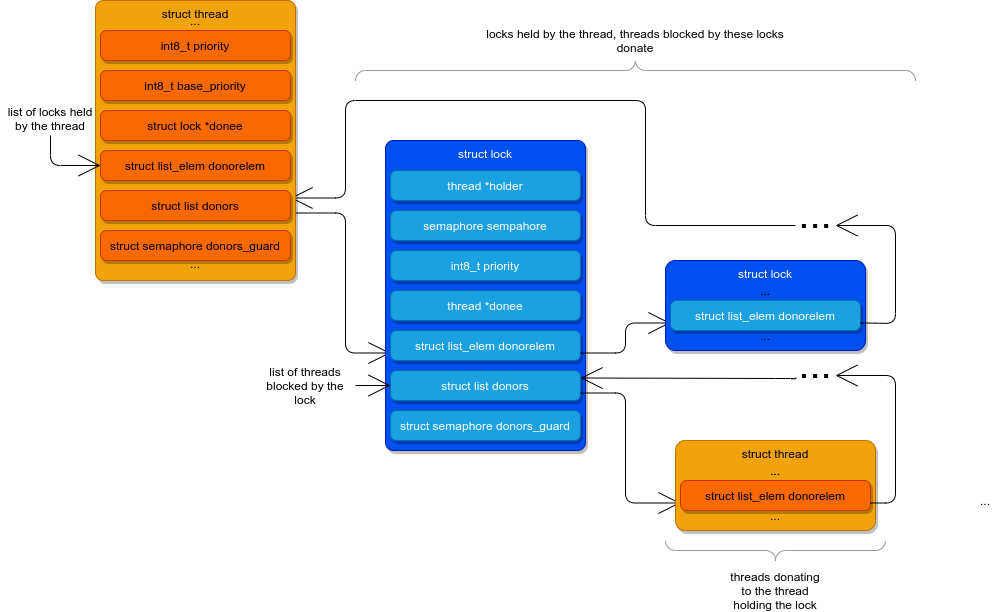
\includegraphics[width=\textwidth]{donation.png}
                \end{center}
                Threads contain a list of donor locks. Each lock contains a list of the threads that are blocked by it.\\
                When a new thread is called \fun{lock\_acquire} and is blocked it is added to the lock's waiters. When a 
                thread is blocked or updates its priority, it calls \fun{donation\_cascading\_update} which propagates its 
                priority to the lock blocking it, and from that lock to the thread holding the lock. This process continues 
                until the max depth or a thread is not blocked by a lock.
                \\ \\ Semaphores are used as guards for threads, to prevent race conditions when updating a thread's priority 
                through donation, or \fun{thread\_set\_priority}. Semaphores are also used to prevent race conditions from 
                occurring when the donors lists of threads or locks are changed as threads are blocked, and start donating 
                their priority.

            \subsection*{Algorithms}

                \subsubsection*{A3  (3 marks) }
                    \question{How do you ensure that the highest priority waiting thread wakes up first for a lock, semaphore, or condition variable?}
                        \begin{itemize}
                            \bullpara{Semaphores}{
                                \\ Locks are implemented using semaphores. \fun{lock\_release} calls \fun{sema\_up} internally,
                                this means locks wake up the highest priority thread the same way semaphores do (see (ii)).
                            }
                            \bullpara{Locks}{
                                \\ Sempahores store the list of waiting threads \struct{semaphore.waiters}. When \fun{sema\_up} 
                                is called, if the waiters list is not empty we then get the \fun{list\_max} of the waiters. 
                                We use \fun{priority\_cmp} as the comparison function to get the highest priority waiter.
                                \\
                                \\ Interrupts are disabled inside semaphores to prevent potential race conditions.
                                \pintoscode{118}{124}{synch.c}{synch.c}
                                (The semaphore wakes the highest priority waiter when signalled)
                            }
                            \bullpara{Condition Variables}{
                               \\A condition variable also stores the list of waiting threads \struct{condition.waiters}. 
                               When \fun{cond\_broadcast} is called, the condition variable is repeatedly signalled until 
                               there are no waiting threads. When signalled (\fun{cond\_signal}) the highest priority 
                               waiter is woken and removed from waiters. This means the threads are woken up in order of 
                               their priority.
                                \pintoscode{334}{339}{synch.c}{synch.c}
                                (The condition variable wakes the highest priority waiter when signalled)
                            }
                        \end{itemize}

                \subsubsection*{A4  (3 marks)}
                    \question{Describe the sequence of events when a call to \fun{lock\_acquire} causes a priority donation. 
                    \\
                    \\How is nested donation handled?} 
                    \\
                    When \fun{lock\_acquire} is called we check the variable \var{donation\_initialised} to see if we need to deal with 
                    priority donation. If the value is set to true then we call the function \fun{donation\_thread\_acquire} 
                    passing in the lock and acquiring thread. 
                    \\ 
                    \\ This function sets the donee of the lock as the thread. 
                    Next, the lock is added to the threads donors queue which holds all the locks donating priority to 
                    the thread. This function then calls \fun{donation\_cascading\_update} passing in the lock. 
                    \\ 
                    \\ This function 
                    handles the updating of priorities. It traverses down the chain of locks and threads until it reaches the 
                    \const{DONATION\_MAX\_DEPTH} or cannot go any further. It updates the threads and locks with a new priority if 
                    their current priority is smaller than the largest donating threads priority.
                \subsubsection*{A5  (3 marks)}
                    \question{Describe the sequence of events when \fun{lock\_release} is called on a lock that a higher-priority thread is waiting for.} 
                    \\ After checking that the current thread holds the lock with an assert, we call \fun{donation\_thread\_release} 
                    passing in the lock. The thread is removed as the donee of the lock and has the lock removed from its donors list.
                    \\ \\
                    \fun{donation\_thread\_update\_donee} then updates the thread's priority to the maximum of the \struct{base\_priority} 
                    of the thread and all the priorities still being donated.
                    \\ \\ The lock is now released, and the highest priority waiter on the lock can now acquire it.
                    We use semaphores as guards on both the lock and the thread, releasing it to prevent race conditions.
            \subsection*{Synchronisation}
                \subsubsection*{A6  (2 marks)}
                    \question{How do you avoid a race condition in \fun{thread\_set\_priority} when a thread needs to recompute its effective priority, but the donated priorities potentially change during the computation?
                    \\
                    \\Can you use a lock to avoid the race?}
                    \\The whole of the donation system hinges on the idea that, between the donees' guards being free, 
                    the list of donees for each node (thread/lock) is always ordered.
                    This enforces some of the synchronisation requirements on the fields of the nodes which are: 
                    \\ \\When changing the priority, we need to hold the
                    semaphore for the node's donors list and its donee's donors list. This is required by the fact 
                    that to update the priority, 
                    we need to get the largest donor from the node and after updating it we need to update that information 
                    in the donee's donors list. This is so our invariant holds. 
                    \\ \\ Similarly, the donors list requires its node's guard to be acquired. The list elem representing 
                    a donor entry in the node's
                    donee's donors list also requires a guard of the node's donee. The donee pointer of the node does not need 
                    to be protected, since it can only be
                    changed by the thread that corresponds to it (if the node is a thread), or by the thread that is 
                    currently holding the lock (if the node is a lock).
                    This way, in order to update the node's priority in \fun{donation\_update\_priority}, called by the 
                    \fun{thread\_set\_priority}, we only need to acquire the node's own donors list guard.

            \subsection*{Rationale}
                \subsubsection*{A7  (3 marks)}
                    \question{Why did you choose this design? In what ways is it superior to another design you considered?}
                    This design uses a simple implementation and it has good speeds for the system loads that pintos can experience with its memory limits.
                    It also handles circular dependencies due to the close interleaving of the code in the very core of the operating system well.
                    \begin{itemize}
                        \bullpara{Naïve approach}{
                            \\ The first design we considered was that every time a priority needed to be fetched, we would go through the whole donation tree of threads 
                            that were donating to that node both directly or indirectly and take the maximum of all base priorities of those threads. We rejected this design
                            from the get-go. 
                            \\ \\ The main issue with this approach is that, although its theoretical worst-case complexity is 
                            technically the same as the complexity of ours, once we add the optimization that we only update 8 levels deep into the priority donation,
                            the number of threads that need to be accessed to update the top thread grows exponentially. Apart from that,
                            the synchronisation cannot be directly hand-over-hand, which further slows down the code by not providing the same amount of fine-grained
                            locking.
                        }
                        \bullpara{Link-cut trees}{
                            \\ The primary problems of this solution are it being more complicated, requiring more testing and having more points of failure that
                            could potentially cause the development not to be completed before the deadline. 
                            \\ \\ Another non-obvious problem with this approach is
                            the complexity constant of link-cut trees[2,3]. This is due to the usage of splays[1] which although fast are still slower than if we limit our depth of
                            priority update. Moreover, due to the need to use either a list-based priority queue or a splay one, it further slows it down over
                            a simple for-loop of several iterations.
                        }
                        \bullpara{Backend for Priority Queue}{
                            \\ We also had to choose the backend for the priority queue used in the nodes of the donation tree. We first settled on a heap-based approach
                            which turned out to be flawed because of the circular dependency of locks used in a \fun{malloc}. This would have been used in the heap,
                            which would have been used by the donation system, which in turn was used by the locks. 
                            \\ \\ We then considered using splay trees[1] but
                            like with the link-cut trees it could potentially have a higher run time over a linked list for the loads expected. This is due to more code and more branching,
                            preventing good pipelining in the CPU. On top of that, it would require more code complexity, which could in turn hinder our ability to deliver the code
                            on schedule.
                        }
                    \end{itemize}

    \section*{Advanced Scheduler}

        \subsection*{Data Structures}
            \subsubsection*{B1  (2 marks)}
                \question{Copy here the declaration of each new or changed `struct' or `struct' member, global or static variable, `typedef', or enumeration. 
                \\
                \\ Identify the purpose of each in roughly 25 words.}
                % Fixed32 struct Code
                \pintoscode{17}{19}{fixed-point.h}{../lib/kernel/fixed-point.h}
                The \struct{fixed32} struct is used to wrap an int value. This can then be used in fixed-point arithmetic. 
                We decided to wrap it in a struct so the C compiler would enforce strong type checking. In this way, an int 
                is never conflated with a \struct{fixed32}, and a \struct{fixed32} is never conflated with an int.
                
                % Thread struct Code
                \pintoscode{91}{123}{thread.h}{thread.h}
                For MLFQS, \struct{thread} was changed to add the variables \var{nice} and \var{recent\_cpu}. These are added to a union 
                with the data used in priority donation. These new entries are to be used in the multi-level feedback queue 
                scheduler. This saves space in the size of \struct{thread}.

                % thread_mlfqs flag
                \pintoscode{137}{137}{thread.h}{thread.h}
                If \var{thread\_mlfqs} is false (default) then we use the round-robin scheduler. Otherwise we 
                use the multi-level feedback queue scheduler described in the PintOS specification.
               
                % load average variable
                \pintoscode{72}{72}{thread.c}{thread.c}
                \var{load\_average} describes the estimate for the average number of ready threads over the last minute. 
                It is calculated using the equations shown in the spec and then used in calculating \var{recent\_cpu}.
                
                % ready_queue_array
                \pintoscode{68}{69}{thread.c}{thread.c}
                \var{ready\_queue\_array} stores a \struct{ready\_queue} for each of the possible priorities. The priority 
                of a ready queue at \var{index} is (\var{index} + \const{PRI\_MIN}).
                
                % num ready threads
                \pintoscode{62}{63}{thread.c}{thread.c}
                \var{num\_ready\_threads} keeps track of the current number of ready threads that are currently waiting for CPU time. 
                This is used for calculating \var{load\_avg} as described in the PintOS specification.
                
                % nonempty ready queues
                \pintoscode{65}{66}{thread.c}{thread.c}
                \var{non\_empty\_thread\_queues} is a list of all the non-empty thread queues stored in order of ascending 
                priority. We can then poll the highest priority ready thread in constant time.

                % Ready struct
                \pintoscode{125}{131}{thread.h}{thread.h}
                \struct{ready\_queue} binds the ready queue for a certain priority, and a list elem so it may be placed 
                in the \var{non\_empty\_thread\_queues} and \var{ready\_queue\_array} structures.
                

        \subsection*{Algorithms}

            \subsubsection*{B2  (3 marks)}
                \question{Suppose threads A, B, and C have nice values 0, 1, and 2 and each has a \var{recent\_cpu} value of 0. 
                \\
                \\Fill in the table below showing the scheduling decision, the priority and the \var{recent\_cpu} values for each thread after each given number of timer ticks:}
            \begin{center}
                \begin{tabular}{l c c c c c c c}
                    timer & \multicolumn{3}{c}{recent\_cpu} & \multicolumn{3}{c}{priority} & thread \\
                    ticks & A & B & C & A & B & C & to run  \\
                    0 & 0 & 0 & 0 & 63 & 61 & 59 & A \\
                    4 & 4 & 0 & 0 & 62 & 61 & 59 & A \\
                    8 & 8 & 0 & 0 & 61 & 61 & 59 & B \\
                    12 & 8 & 4 & 0 & 61 & 60 & 59 & A \\
                    16 & 12 & 4 & 0 & 60 & 60 & 59 & B \\
                    20 & 12 & 8 & 0 & 60 & 59 & 59 & A \\
                    24 & 16 & 8 & 0 & 59 & 59 & 59 & C \\
                    28 & 16 & 8 & 4 & 59 & 59 & 58 & B \\
                    32 & 16 & 12 & 4 & 59 & 58 & 58 & A \\
                    36 & 20 & 12 & 4 & 58 & 58 & 58 & C \\
                \end{tabular}
            \end{center}

            \subsubsection*{B3  (2 marks) }
                \question{Did any ambiguities in the scheduler specification make values in the table uncertain? 
                \\ \\ If so, what rule did you use to resolve them?}
                \\ When more than one thread has the highest priority, they are scheduled in a round-robin scheme.
                \\ \\ When the highest priority thread has its priority reduced to that of another (or more) threads, 
                it is moved to a new ready queue and where it should be added in the ready queue is ambiguous.
                \begin{center}
                    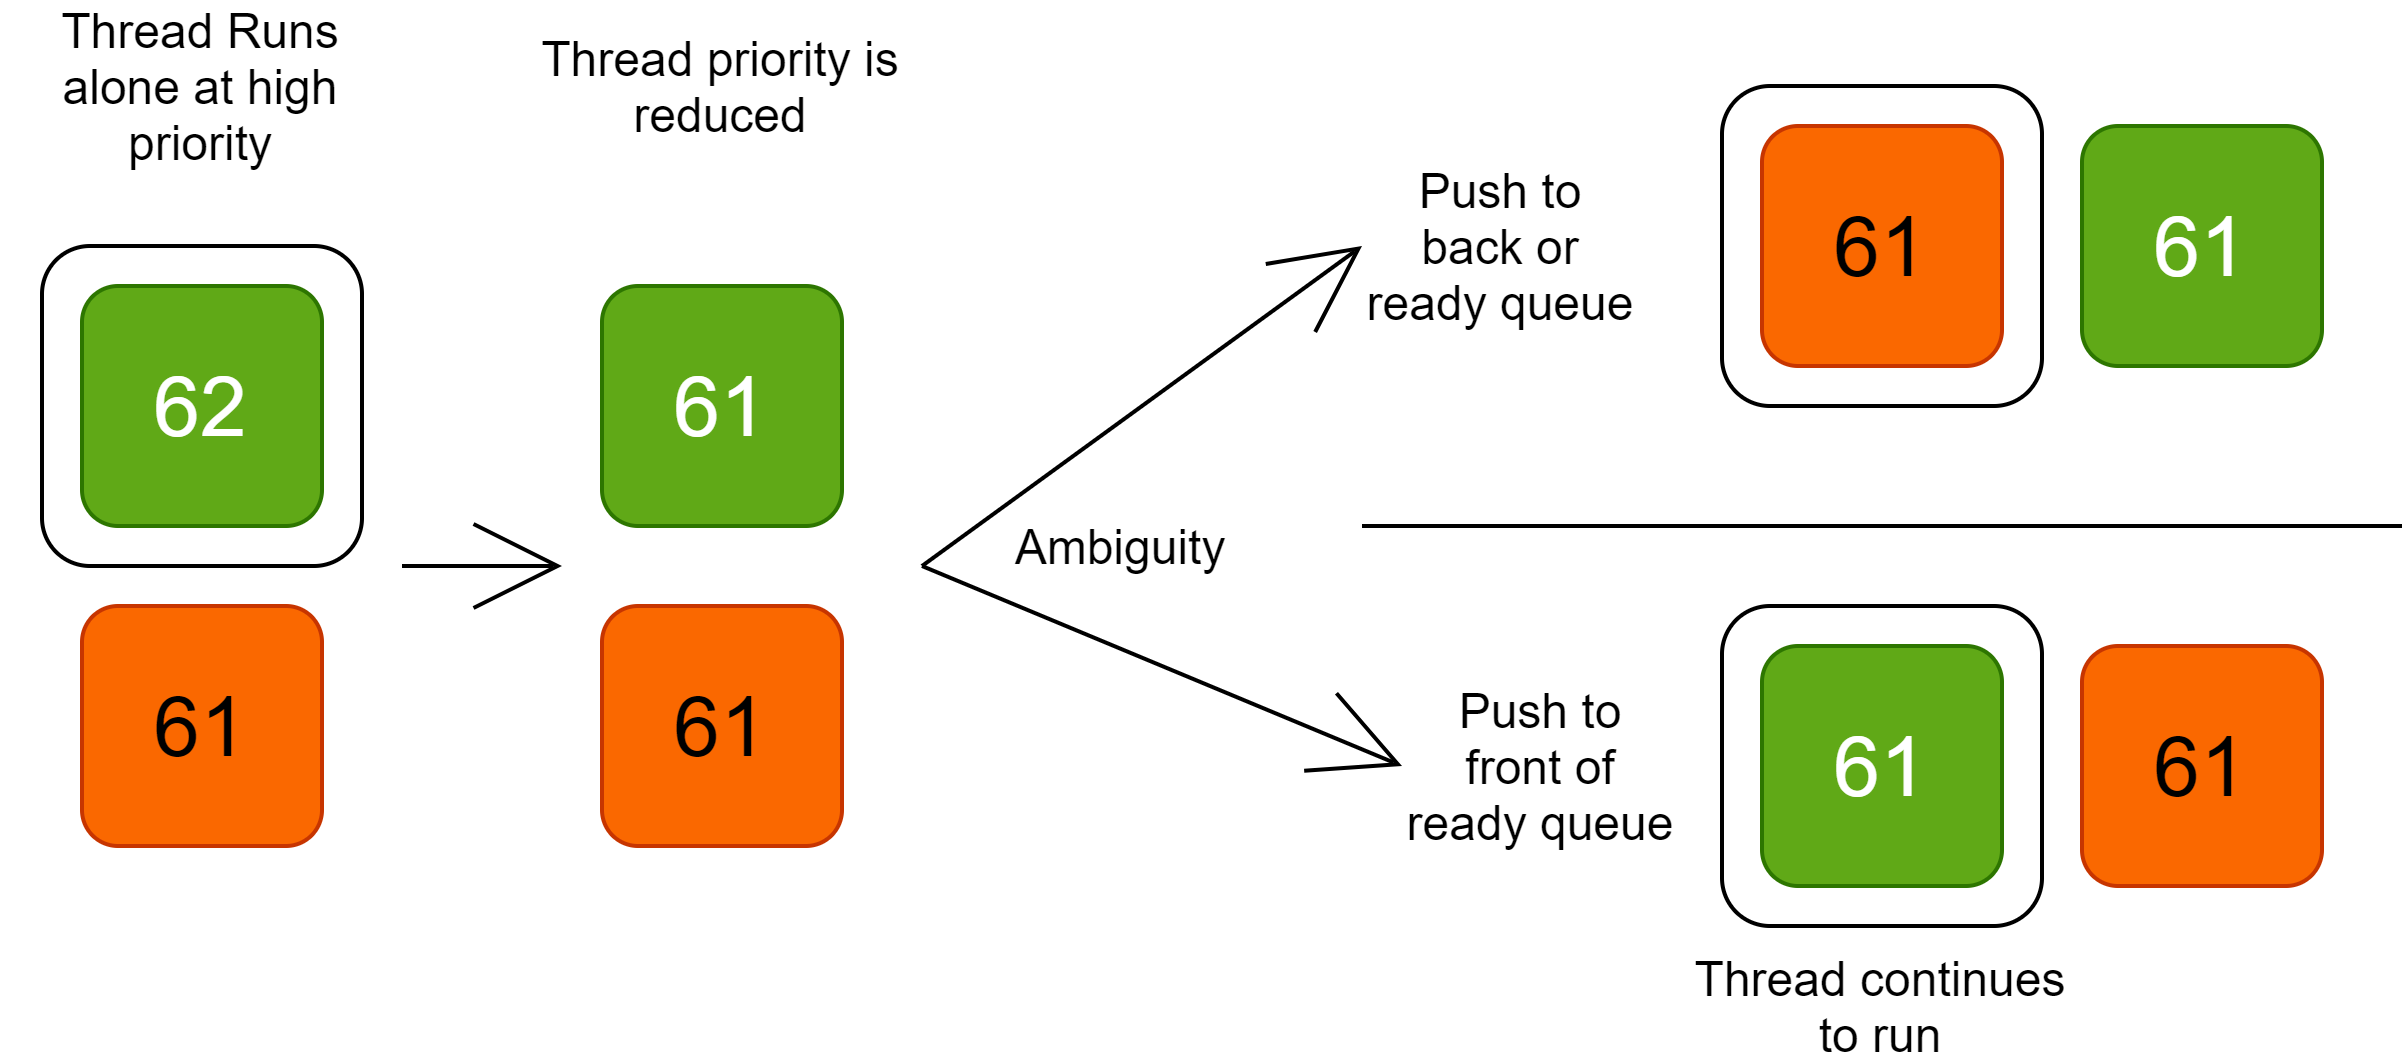
\includegraphics[width=\textwidth]{ambiguity.png}
                \end{center}
                We decide to continue running a thread so long as its priority is greater than or equal to the highest 
                priority of the other ready threads. When the thread yields it is inserted to the back of the ready queue associated 
                with its priority.
                \\ \\ As a result, on the table when thread \keyword{A} is demoted from $62 \to 61$ it continues to 
                be run until the time slice is over (it still has the highest priority). It then ends up at the back of 
                the ready queue from priority $61$, allowing \keyword{B} to be run.


        \subsection*{Rationale}

            \subsubsection*{B4  (3 marks)}
                \question{Briefly critique your design, pointing out advantages and disadvantages in your design choices.}
                \\ Our implementation of fixed-point operations works by the following. There is a struct \struct{fixed32} 
                that stores a single element. The value should not be modified but instead, new \struct{fixed32} structs 
                should be initialized with the modified value. This makes the fixed point operations more complicated 
                but has the added benefit that we can never confuse a fixed point value for an integer. If \struct{fixed32} 
                was a typedef of an integer, the C compiler would allow us to implicitly cast it to an integer. This would 
                cause logical errors. This implementation allows us to do calculations between \struct{fixed32} values 
                and integers with added safety. This implementation has worked well for us.
                
                \begin{center}
                    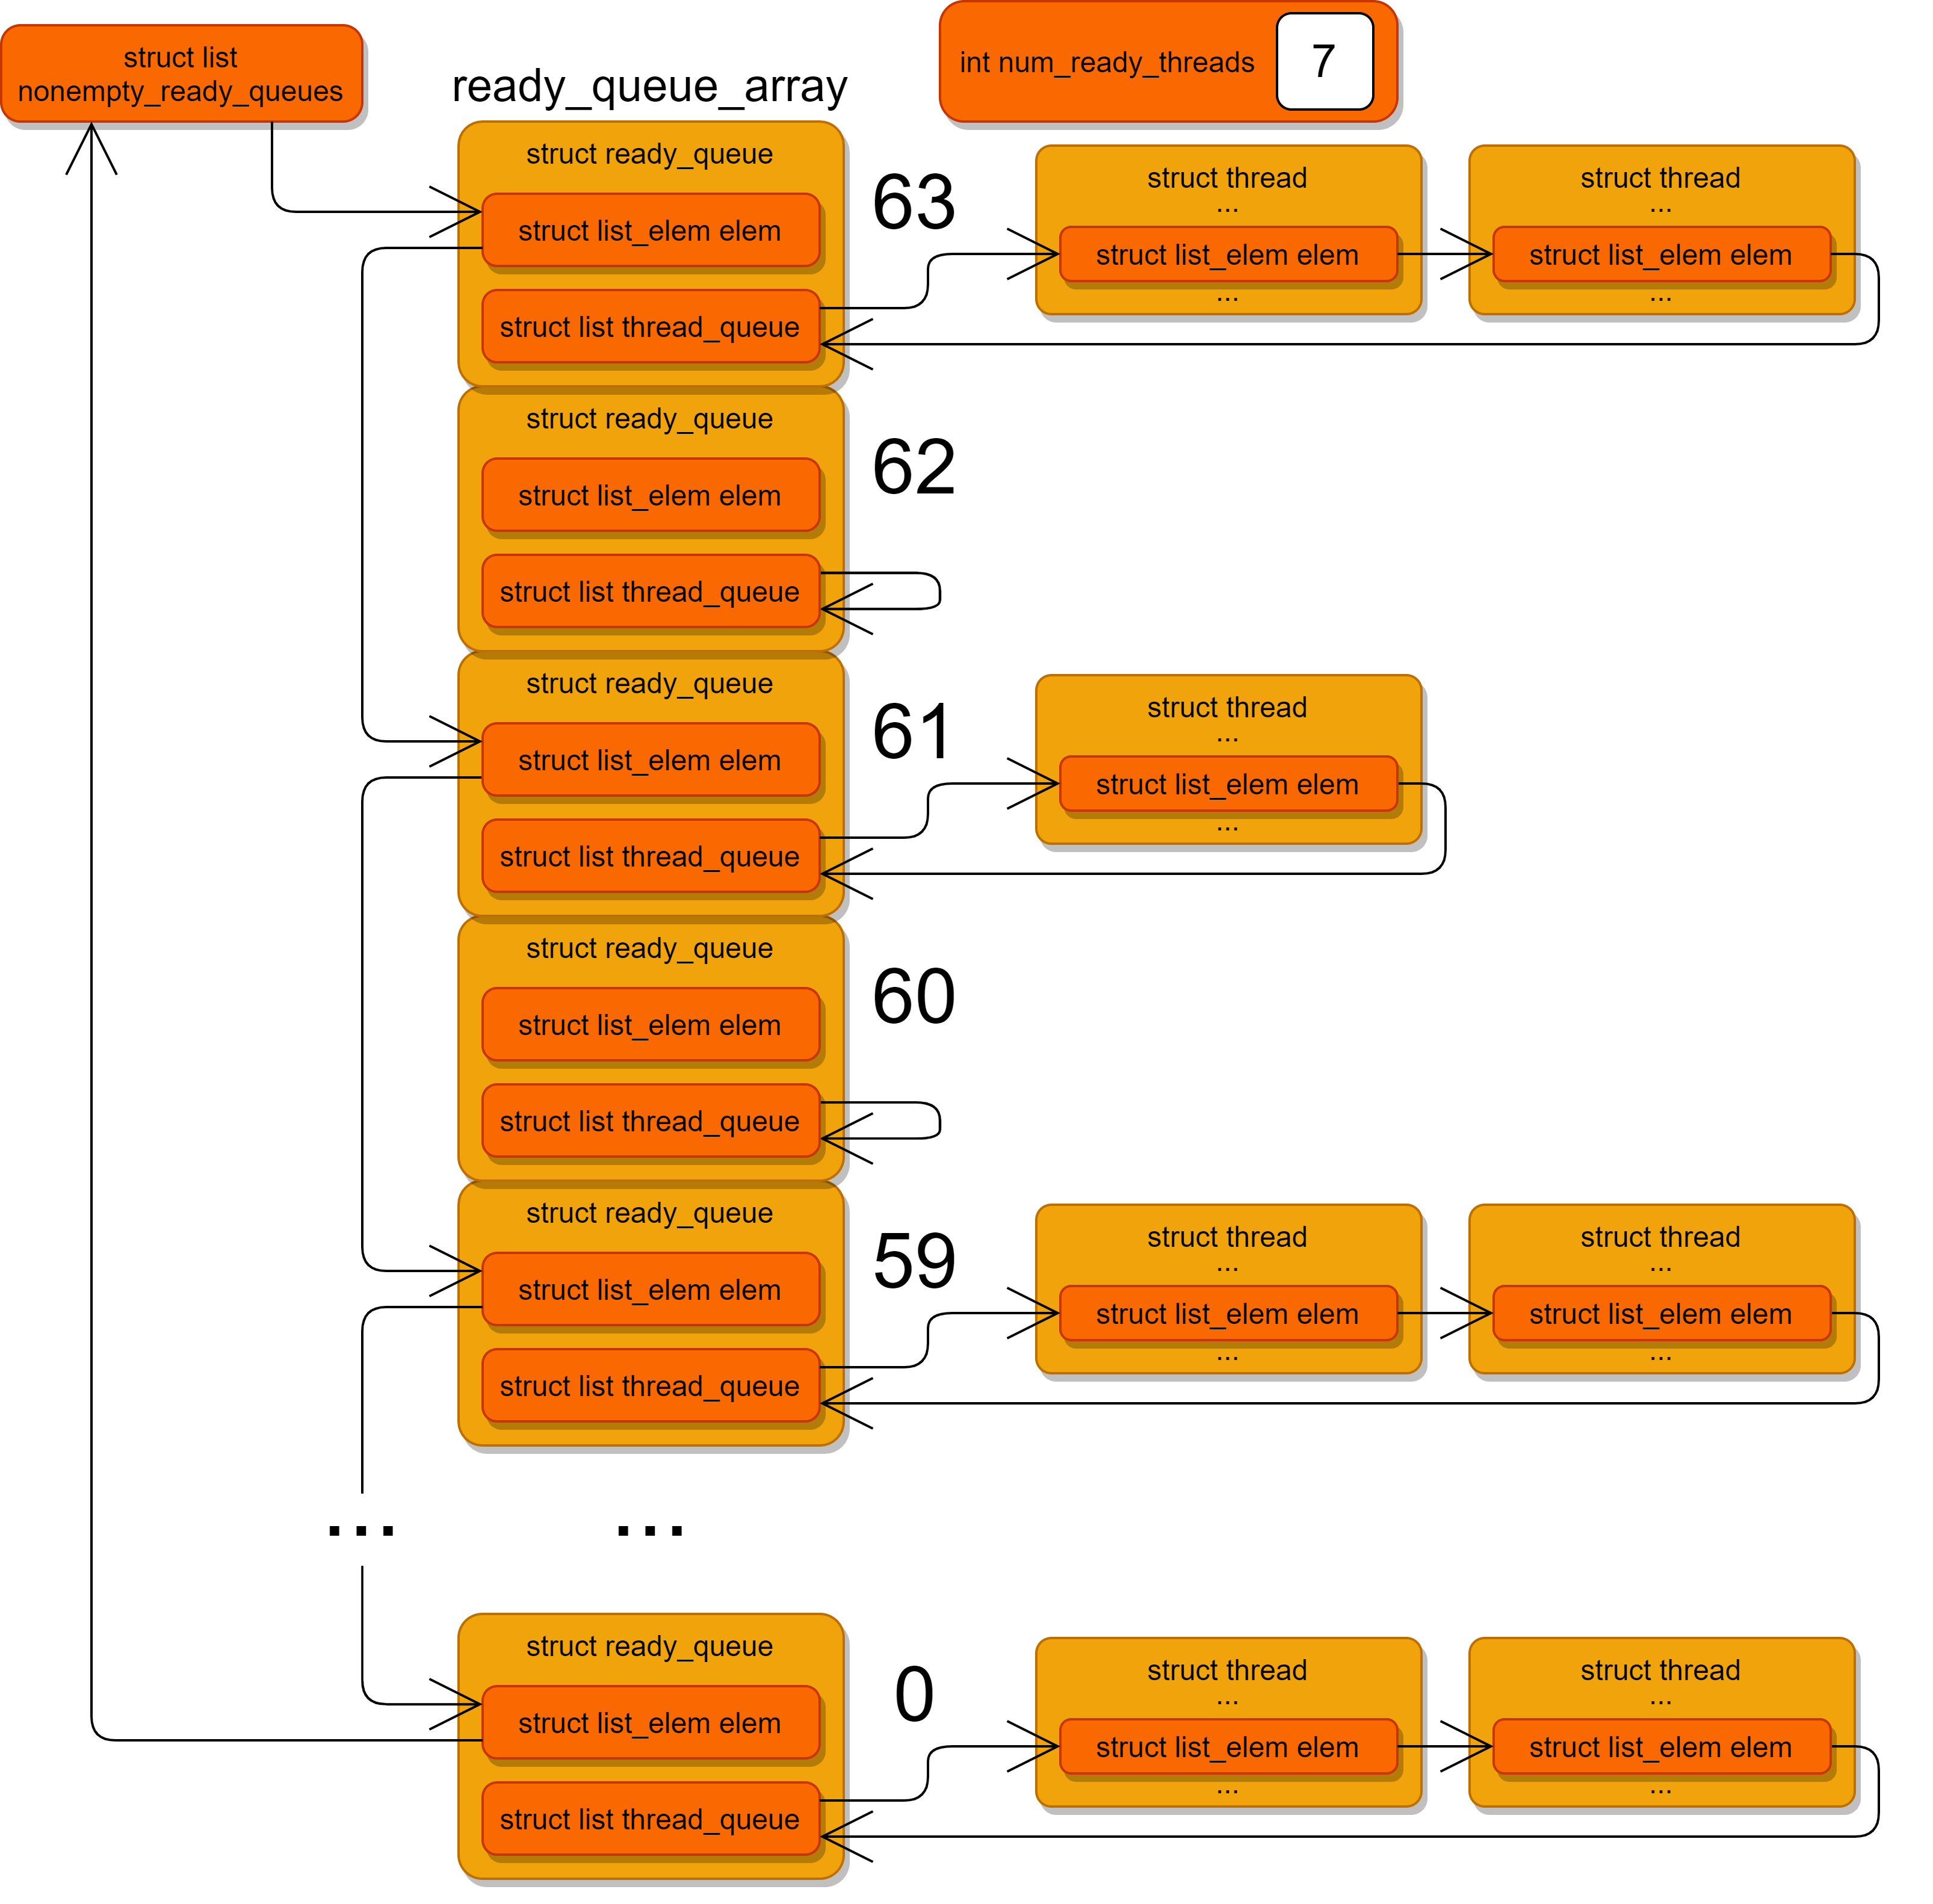
\includegraphics[width=\textwidth]{scheduler.png}
                \end{center}
                We implemented the scheduler using an array of 64 \struct{ready\_queue}s, the index of the ready queue 
                is equivalent to its priority. Every thread with status \const{THREAD\_READY} is present in this system.
                \\ \\ All non-empty ready queues were then linked together in a list, ordered by descending priority.
                \\ \\ This approach had several advantages:
                \begin{itemize}
                    \bullpara{Insertion is fast}{
                        \\ To insert a thread requires only three steps in \fun{ready\_add}:
                        \begin{enumerate}
                            \item \fun{list\_push\_back} the thread on the ready queue at the index of its priority.
                            \item If the list was previously empty, insert the ready queue into the non-empty ready queues. 
                            Our comparison function can use the memory location of the ready queue struct's \struct{list\_elem} 
                            directly for this.
                            \item Increment \var{num\_ready\_threads}.
                        \end{enumerate}
                        As a result, the worst case scenario is when priorities $63 \to 1$ have at least one thread, 
                        priority $0$ is empty, and we insert one thread into priority $0$. This would require a traversal 
                        over $63$ list elements with $63$ direct comparisons of pointers.
                    }
                    \bullpara{Removal is fast}{
                        \\ To remove a thread requires only three steps in \fun{ready\_remove}:
                        \begin{enumerate}
                            \item Use \fun{list\_elem\_alone} to determine if the thread is the last in its ready queue. 
                            If so use \fun{get\_list} to get the ready queue it is in, and \fun{list\_remove} it from the 
                            non-empty ready lists.
                            \item Call \fun{list\_remove} on the threads \struct{list\_elem}.
                            \item Decrement \var{num\_ready\_threads}.
                        \end{enumerate}
                        The worst case for this is when the only thread of a ready queue is removed. This is still very 
                        fast as \fun{list\_elem\_alone} only checks two pointer values. \fun{get\_list} is very fast when 
                        there is a single element, and \fun{list\_remove} simply connects its adjacent elements by copying pointers.
                    }
                    \bullpara{Updating thread positions is fast}{
                        \\ Updating a thread's position requires a \fun{ready\_remove} followed by a \fun{ready\_add}. As
                         both are fast, so too are updates.
                    }
                    \bullpara{Getting the next thread is fast}{
                        \\ We can simply take the first element of the first ready queue in \var{nonempty\_ready\_queues}.
                    }
                    \bullpara{Getting size is fast}{
                        \\ As we use an \struct{int} to keep track of the number of ready threads, we do not need to interact 
                        with our thread queue structure at all to get its size.
                    }
                    \bullpara{It is flexible}{
                        \\ The size of the \var{ready\_queue\_array} is based off \const{PRI\_MIN} and \const{PRI\_MAX}, 
                        as is \fun{ready\_add}. This means priorities can be changed (e.g $\text{\const{PRI\_MIN}} = 42$) 
                        without causing issues.
                    }
                \end{itemize}
                \textbf{The disadvantage - additions to \file{list.h}:}
                \\ To allow for fast removal of threads without traversing the list or making assumptions about a thread's 
                priority, we must be able to remove the \struct{ready\_queue} it is contained in using the thread's 
                \struct{list\_elem}. 
                \\ \\ To achieve this without exposing \file{thread.c} to the internal workings of \file{list.c} we added 
                two new functions to \file{list.c}. 
                \pintoscode{316}{320}{list.c}{../lib/kernel/list.c}
                \pintoscode{288}{295}{list.c}{../lib/kernel/list.c}
\end{document}
